% ╒══════════════════════════════════════════════════════════════════════════╕ %
% │                                CHAPTER  1                                │ %
% ╘══════════════════════════════════════════════════════════════════════════╛ %
\ifdm
    \chapter{Concept}
    \label{concept}

    \DndDropCapLine{A}{n \Subclass{} \Class{}} \Race{}. Cold \& calculated from nature \Name{} still shows a lot of emotions for a \Race. Trying to release her master, \MasterFullName{}, who was cursed and turned into a spellbook.

    \section{\Race{}} 
    \Race{} are fey creatures following the lesser deity the Raven Queen and living in the Shadow Realm. \Name{} hasn't lived long in the Shadow Realm and has no memory of this time. It still slightly touched his personality to be somewhat more cold and calculated than most. Unlike most of his kin, he however has more emotions and do not take sick pleasure out of pain.

    \subsection{Emotions}
    As mentioned before, \Name{} is noticeably more cold than most people. He still feels joy, happiness and sadness just like any other non-influenced human or creature. You can notice that he still cares a lot, by him trying to release \Master{} and being upset that he she is a bit more pale.

    As \Name{} is not aware that he/she is a \Race{} and gets upset when people mistake her for anything else then a kind of elf. \Name{} is afraid of being a drow, and doesn't even know of the existence of \Race{}.

    \vfill
    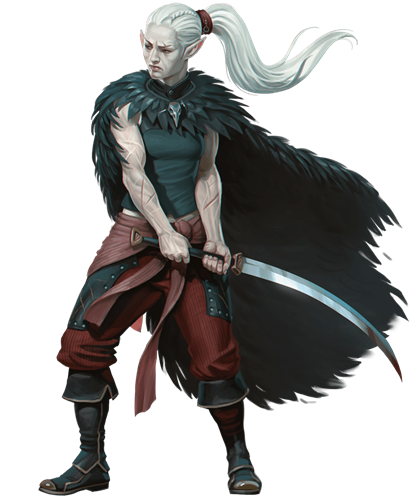
\includegraphics[width=\linewidth-2ex]{images/shadar-kai.png}
    \vfill
    \newpage
  
    \section{Profession}
    As \Name{} is \Master{} apprentice, he is trying to become a full-blown \Class{}. Sprinkled with some craftiness, especially for the arcane.

    \section{Personality}
    As mentioned before in the Race section, \Name{} is a tad more cold and calculated, whilst still being very sensitive on his/her looks as a 'drow' or other kind of elf. He/she gets upsets when mistaken for anything else then a 'normal' elf.

    \subsection{Quirks}
    Gets upset when you mistake her for a drow

    \section{Background concept}
    \begin{itemize}
        \item Unbeknown to \Name{}, adopted by parents
        \item \Mom{} found \Name{} in abandon temple, convinced \Dad{} to adopt/keep.
        \item \Name{} always had a hunger learn new things \& make discoveries
        \item \Name{} Showed a talent for memorizing
        \item \MasterFullName{} approached parents recognizing the talent
        \item \Name{} studied magic under \Master{}
        \item \Master{} was a high ranking member of \CloisterIntro{}
        \item \Name{} didn't mind going the extra mile to discover new magical abilities \& lore
        \item \Master disappeared one day, \Name{} found out after a while he was cursed and turned in a book
        \item \Name{} found clues to release his teacher from the curse.
        \item \Name{} set on a quest to lift the curse by filling the spellbook
        \item The Raven Queen is behind the curse
        \item On the quest \Name{} got captured and woke up in the arena
      \end{itemize}
      

    \subsection{Bonds \& Goals}
    \begin{itemize}
        \item Somehow bound to the Raven queen. Unknown to \Name{} though
        \item Wants to lift the curse on \MasterFullName{}
        \item Is very protective over her race and her parents
        \item Has a hunger for magical lore \& discoveries, especially lost or hidden ones.
        \item Dreams of opening his own school/library
        \item Doesn't want comfort, but is motivated by gold as a means to the goal
    \end{itemize}

    \subsection{Notable Relations}
    \begin{itemize}
        \item Mother \& Father are dear
        \item Respects \Master{} and his magical capabilities
        \item Has a good relationship with \CloisterIntro{}, because of the teacher
    \end{itemize}

    \section{Aimed progression \& Goals}
    \begin{itemize}
        \item Wants to discover lost and hidden magic
        \item Wants to gather a butt-load of spells
        \item Wants to be a master spell crafter
        \item Wants to have unique/hidden spells where the usage is a big surprise
        \item Wants to have his own (magic) library/school
        \item Wants to set \Master{} free
        \item \bookauthor{} wants the race issue to come up and for \Name{} to discover their origin \& relation to The Raven Queen / Shadow Realm
        \item \bookauthor{} will probably make \Name{} a full \Class{} without multi-classing.
    \end{itemize}

    \section{Appearance}

\fi